\chapter{Two protocols based on Spekkens contextuality}
\label{sec:protocols}
We now generalize the self-testing result in \cite{Bharti2019}, which was discussed in Section \ref{sec:contselftesting}, to the framework of Spekkens contextuality. In particular, this will lift the usual restriction to noise-free projective measurements. Additional features will be discussed in Section \ref{sec:discussion}. The first protocol we will consider assumes approximate operational equivalences for some preparations, as well as a bounded information carrying capacity, much like the protocol in Section \ref{sec:contselftesting}. In Section \ref{sec:relaxmemoryass}, we will study how imposing additional constraints, in terms of operational equivalences, on the measurement devices allows us to relax this memory assumption.
\section{Self-testing from approximately operationally equivalent preparations and bounded memory}
Let $n\geq 5$ be an odd integer. The protocol we consider is reminiscent of the ideal $n$-cycle reference experiment \ref{eqn:ncycleideal}. As such, we assume an experimenter to be able to freely choose between $n$ three-outcome measurements $\{M_i\}_{i=1}^n$ with outcomes $m_1$, $m_2$, $m_3$. We assume measurements to be chosen according to a uniform distribution and denote measurement events by  $m_k\thinspace\vert\thinspace M_i$, or $m_k,m_l\thinspace\vert\thinspace M_i,M_j$ for two sequential measurements. As shown in Figure \ref{fig:ncycleselftesting}, for ideally operating devices, the measurement events $m_1 \thinspace\vert\thinspace M_i$ correspond to the rank-one projectors $\vert u_i^{(n)}\rangle\langle u_i^{(n)}\vert$, defined by \ref{eqn:ncycleideal}. Further, in the ideal case, the measurement events $m_3\thinspace\vert\thinspace M_i\equiv m_1\thinspace\vert\thinspace M_{i\oplus 1}\equiv\vert u_{i\oplus 1}^{(n)}\rangle\langle u_{i\oplus 1}^{(n)}\vert$ and the events $m_2\thinspace\vert\thinspace M_i$ correspond to the projectors $\mathbb{1}-\vert u_i^{(n)}\rangle\langle u_i^{(n)}\vert-\vert u_{i\oplus 1}^{(n)}\rangle\langle u_{i\oplus 1}^{(n)}\vert$ onto the pure qutrit state completing the orthogonal triad $\subset \mathbb{C}^3$. In Figure \ref{fig:ncycleselftesting}, the events $m_3\thinspace \vert\thinspace M_i$ and $m_1\thinspace\vert\thinspace M_{i\oplus 1}$ are non-overlapping, despite corresponding to the same ideal projectors, to highlight that we do not need to assume operational equivalence.

\begin{figure}
	\begin{subfigure}[t]{0.45\textwidth}
    	\centering
    	\includegraphics[width=\textwidth]{images/mntsandpreps.png}
        \caption{}
	\end{subfigure}
	\hfill
    \begin{subfigure}[t]{0.45\textwidth}
    	\centering 
        \includegraphics[width=0.8\textwidth]{images/kcbsrefstates.png}
        \caption{}
    \end{subfigure}
    \caption{\textbf{(a):} Measurement events and retrospective preparations corresponding to a self-testing scenario consistent with cycle length $n=5$. The experimenter can choose from five three-outcome measurements $M_i$, with outcomes $\{m_1,m_2,m_3\}$. In post-processing, the experimenter defines $2n$ preparations $\{P_{m_k\vert M_i}\}_{k,i}$, for $k\in\{1,2\}$ and $i\in\{1,\dots,n\}$. We define $P_{m_3\vert M_i}\coloneqq P_{m_1\vert M_{\oplus 1}}$. In the ideal case, the measurement events $\{m_k\vert M_i\}_{k\in\{1,2,3\}}$ correspond to rank-one projectors onto the orthogonal triad $\subset \mathbb{C}^3$ containing the cycle states $\vert u_i\rangle$ and $\vert u_{i\oplus 1}\rangle$. Furthermore, in the ideal case, the preparations $P_{m_k\vert M_i}$ are pure states that coincide with the vectors in this triad. The measurement events $m_3\vert M_i$ and $m_1\vert M_{i\oplus 1}$ are non-overlapping to illustrate that the self-testing protocol does not assume operational equivalence of these, despite the fact that they correspond to the same rank-one projector onto $\vert u_{i\oplus 1}\rangle$ in the ideal case. \textbf{(b):} Juxtaposition with the cycle states belonging to the odd $n$-cycle scenario for $n=5$. Figure (a) can be seen as a top view of (b), with every black dot corresponding to a cycle state $\vert u_i\rangle$.}
\label{fig:ncycleselftesting}
\end{figure}

Like in Section \ref{sec:contselftesting}, we assume i.i.d.\ rounds, i.e. the devices to operate in an identical manner for all rounds of the protocol, in particular independently of previous input-output cycles. This allows us to lift relative frequencies to probabilities. We will discuss all other assumptions in due time. The protocol consists of the following steps:
\begin{enumerate}
\item The experimenter prepares the system in a distinguished preparation $P_0$ by selecting the appropriate setting on the corresponding device.
\item The experimenter samples from a uniform distribution and selects two integers $(i,j)\in\{1,\dots,n\}^2$ at random.
\item The experimenter performs the measurements $M_i$, $M_j$ in sequence, first $M_i$, then $M_j$. He does so by selecting the correct settings on the corresponding devices and records the outcomes.
\item Steps 1-3 are repeated to obtain estimates for the probability distributions \\ $p((m_k,m_l)\thinspace\vert\thinspace (M_i,M_j),P_0)$. 
\item Additionally, the experimenter performs single measurements on two auxilliary preparations $P_1$ and $P_2$ he can choose from and obtains estimates for the probability distributions $p(m_k\thinspace\vert\thinspace M,i, P_j)$, for $j\in{1,2}$.
\item Post-processing
	\begin{enumerate}
	\item Certificate of quantumness
	\item Bounding compatible quantum models
	\end{enumerate}
\end{enumerate}

We write the free choice of measurements $(M_i,M_j)$ and subsequent outcomes $(m_k,m_l)$ as ordered lists to indicate that the distributions $p((m_k,m_l)\thinspace\vert\thinspace (M_i,M_j),P_0)$ are in general not independent of the order, since we do not assume any underlying compatibility relations, like we did in Section \ref{sec:contselftesting}. In the ideal case, the distinguished preparation $P_0$ corresponds to the $\ket{0}$ qutrit state, which produces a maximal violation of the KCBS inequality. Additionally, we assume access to two additional auxilliary preparations, $P_1$ and $P_2$, which we require to establish approximate operational equivalences during post-processing. In the ideal case the preparations $P_1$ and $P_2$ correspond to the $\ket{1}$ and $\ket{2}$ qutrit states, forming an orthogonal triad with $\ket{0}$. The convex combination $\frac{1}{3}\sum_{i=0}^2 P_i\equiv\frac{1}{3}\sum_{i=0}^2\ket{i}\bra{i}=\frac{\mathbb{1}}{3}$ corresponds to the fully mixed state $\frac{\mathbb{1}}{3}$, as does the convex combination with equal weights of the ideal projectors corresponding to the measurement events $\{m_k\vert M_i\}_{k=1}^3$, for all $i\in\{1,\dots,n\}$. Here, we implicitly defined the convex combination of two preparations to be the preparation that is implemented by generating a random number and performing the preparation procedure associated with that outcome. We note that Steps 1-4 of the protocol correspond almost one-to-one to the steps of the protocol in \cite{Bharti2019}, which was discussed in Section \ref{sec:contselftesting}, the only difference being that the experimenter now freely chooses between $n^2$, as opposed to $n$ measurement settings.

We now elaborate on Step 6 of the protocol, detailing how an agent may post-process the acquired data, with the goal of self-testing the apparatus. The experimenter retrospectively defines $2n$ preparations, which we denote $P_{m_k\vert M_i}$, for $i\in\{1,\dots,n\}$ and $k\in\{1,2\}$. As suggested by the notation, $P_{m_k\vert M_i}$ is prepared by performing the measurement $M_i$ on a system initially prepared like $P_0$, and conditioning on the outcome $m_k$. We refer to these preparations as retrospective, since they are not directly implemented by the experimenter. However, one can infer the relevant statistics $p(m_k\thinspace\vert\thinspace M_i, P_{m_l\vert M_j})$ for these preparations from the distributions $p((m_k,m_l)\thinspace\vert\thinspace (M_i,M_j))$:
\begin{equation*}
p(m_k\thinspace\vert\thinspace M_i, P_{m_l\vert M_j})=\frac{p((m_k,m_l)\thinspace\vert\thinspace (M_i,M_j))}{\sum_{k'\in\{1,2\}} p((m_{k'},m_l)\thinspace\vert\thinspace (M_i,M_j))}.
\end{equation*}
These retrospective preparations will be used in Section \ref{sec:certifyquant}, where we introduce a criterion to certify the quantumness of the apparatus.

Additionally, the experimenter can infer the statistics $p(m_k\thinspace\vert\thinspace M_i, P_0)$ from the correlations $p((m_k,m_l)\thinspace\vert\thinspace(M_i,M_j),P_0)$:
\begin{equation*}
p(m_k \thinspace\vert\thinspace M_i, P_0)=\sum_{l,j}\frac{1}{n}p((m_k,m_l)\thinspace\vert\thinspace (M_i,M_j),P_0).
\end{equation*}
These will become relevant in Section \ref{sec:boundingmodels}, when bounding the compatible quantum models.
\subsection{Step 6a: Certificate of quantumness}
\label{sec:certifyquant}
By coarse-graining, we obtain $2n$ binary measurements from the $n$ three-outcome measurements $M_i$: for each $M_i$ we ``lump together" the outcomes $m_2$, $m_3$, and $m_1$, $m_3$. In total, we define $2n$ binary measurements and $2n$ preparations during post-processing. We denote the outcomes of the $2n$ binary measurements as $0$, $1$, where the outcome $0$ corresponds to the two coarse-grained measurement events. If we consider the ideal reference experiment \ref{eqn:ncycleideal}, the outcomes $0$, $1$ correspond to the eigenvalues of the rank-one projectors we can associate with each of the binary measurments. There are $n$ ideal binary measurements that probe the probability of finding the system in one of the $n$ one-dimensional subspaces spanned by the $n$ cycle states. The other $n$ ideal binary measurements correspond to rank-one projectors onto states in an orthogonal triad containing two cycle states. For the extent of this subsection we will for simplicity index the $2n$ binary measurements and preparations like $\{M_i\}_{i\in\{1,\dots,2n\}}$ and $\{P_i\}_{i\in\{1,\dots,2n\}}$. For ideal measurements and preparations, we can choose the order such that the ideal measurement $M_i$ is the rank-one projector onto the ideal pure state preparation $P_i$. Therefore, for ideal devices, the retrospective preparations and binary measurements, if ordered in this manner, satisfy \begin{equation}
\label{eqn:epsilon}
\epsilon \coloneqq \max_i p(0\vert M_i, P_i)\stackrel{\text{ideal}}{=}0.
\end{equation} 
For noisy devices, we expect to find an ordering for which \ref{eqn:epsilon} is approximately satisfied, with the parameter $\epsilon$ characterizing the amount of noise. The parameter $\epsilon$ can be determined from the observed statistics during post-processing.

Apart from the noise-characterizing parameter $\epsilon$, the second relevant parameter for certifying quantumness is
\begin{equation*}
\eta\coloneqq \min_{\substack{i,j \\ i\neq j}} p(0\vert M_i, P_j).
\end{equation*}
For quantum devices, the parameter $\eta$ can be thought of as a measuring the maximum overlap or closeness of distinct states. As such, $\eta$ decreases as the cycle length $n$ increases. Let $m=2^k$. In Appendix B of \cite{Pusey2019a} it is proven that for a set of preparations $\{P_i\}_{i=1}^m$ and measurements $\{M_i\}_{i=1}^m$, producing statistics obeying $\epsilon<\frac{1}{4}\eta^2$, to be compatible with a (preparation) non-contextual ontological description, requires at least $k$ binary measurements in any TC set. The intuition behind this is the following: From the statistics of the $m$ preparations $\{P_i\}_{i=1}^m$ one can infer the statistics of any preparation in the convex hull of the $\{P_i\}_{i=1}^m$. If the $m$ preparations are not very ``close", as measured by $\eta$, relative to their sharpness, as measured by $\epsilon$, (this is enforced by the condition $\epsilon<\frac{1}{4}\eta^2$) then the associated probability density functions $\{\mu_i\}_{i=1}^m$ will have non-significant overlap. In particular, if we regard the $m$ probability density functions on the ontic state space $\Lambda$ as vectors $\{v_i\}_{i=1}^m$ in $\mathbb{R}^{\vert \Lambda \vert}$, then the proof in Appendix B of \cite{Pusey2019a} establishes that the $m=2^k$ vectors vary in $k$ linearly independent directions. Demanding preparation non-contextuality, every distinct preparation in the convex hull of the $\{P\}_{i=1}^n$ must produce different predictions for at least one of the measurements in a TC set. Finally, \cite{Pusey2019a} notes that the function mapping a probability density function $\mu_j$, or rather the corresponding vector in $\mathbb{R}^{\vert \Lambda \vert}$ to the probability $p(m_k\thinspace\vert\thinspace M_i,\mu_j)$ of obtaining the outcome $m_k$ when performing the measurement $M_i$ for an initial preparation $\mu_j$ is linear. Hence, such mapping $\mathbb{R}^{\vert \Lambda \vert}\rightarrow\mathbb{R}$ is of the form $(x_1,\dots,x_{\vert \Lambda \vert})\mapsto a_1 x_1+\dots + a_n x_n = \vec{a}\cdot \vec{x}$ with $0 \leq a_i \leq 1$, and $x_i$ the components w.r.t\ the standard basis of $\mathbb{R}^{\vert \Lambda \vert}$. Binary measurements can therefore only distinguish between preparations along a single direction, $\vec{a}$. Preparations whose ontological representations differ w.r.t.\ directions orthogonal to $\vec{a}$, are assigned the same probabilities by the binary measurement characterized by $\vec{a}$. A TC set of measurement must contain at least $k$ binary measurements for $k$ ``linearly independent"` preparations, if we demand compatiblity with a preparation non-contextual ontological model.

We now turn to the bounded memory assumption required by the protocol, which relies on the results of \cite{Pusey2019a}, the relevant ones of which were sketched above. Assume that the experimenter has access to $n\geq 5$ three-outcome measurement settings, like we considered at the beginning of Section \ref{sec:protocols}, where $n$ is odd (think of $n$ as the cycle-length). Further, let $k$ be the largest integer satisfying $2n\geq 2^{k+1}$. To certify quantumness, we assume that there exists a TC set of measurements with $k$ binary measurements, i.e. that $k$ binary measurements are sufficient to fully characterize the statistics of the system at hand. If we find the condition $\epsilon<\frac{1}{4}\eta^2$ to be satisfied, we consider the system to be quantum.  How does this assumption relate to the assumption of bounded memory in Section \ref{sec:memoryass}? If we define the information carrying capacity as 
\begin{equation*}
\mathcal{I}\coloneqq \log_2(\text{number of states that can be perfectly distinguished}),
\end{equation*}
then assuming a TC set with $k$ measurements implies bounding the information carrying capacity: $\mathcal{I}\leq k$ bits. In this sense, assumptions regarding the minimal size of TC sets of measurements directly relate to bounds on the information carrying capacity. In particular, bounding the information carrying capacity $\mathcal{I}\leq k \text{ bits}$ implies a finite-dimensional Hilbert space $\mathcal{H}$, $\operatorname{dim}(\mathcal{H})\leq k$.

If we wish to allow for an information carrying capacity of $k$ bits, we require an apparatus consistent with a cycle length $n$ such that
\begin{alignat*}{2}
& && 2n\geq 2^{k+1} \\
& \iff && \log_2(n)\geq k.
\end{alignat*}
The relationship between cycle length and simulable bound on the information carrying capacity is logarithmic, as was the case for the class of protocols in Section \ref{sec:contselftesting}, which assumed sharp measurements and cyclic compatibility relations. The price one has to pay to account for a greater information carrying capacity is two-fold:
\begin{itemize}
\item the apparatus must include additional measurement settings to be consistent with a greater cycle length $n$
\item for a greater cycle-length $n$, a greater fidelity to the reference experiment is required, since for the ideal odd $n$-cycle scenario the relevant parameter $\frac{1}{4}\eta^2$, which bounds how sharp the measurement implementations must be for self-testing, decreases with an increasing cycle length $n$:
\begin{equation*}
\frac{1}{4}\eta^2 = \frac{1}{2}\left(\frac{\pi}{n}\right)^4.
\end{equation*}
\end{itemize}

\subsection{Step 6b: Bounding compatible quantum models}
\label{sec:boundingmodels}
As discussed in Section \ref{sec:certifyquant}, we assume a Hilbert space of bounded dimension, say $\operatorname{dim}(\mathcal{H})\leq d$. We can w.l.o.g.\ take $\mathcal{H}$ to be $\mathbb{C}^k$, $k\leq d$, where $k$ is the true dimension of $\mathcal{H}$. For notational simplicity we define $P_{m_3\vert M_i}\coloneqq P_{m_1\vert M_{i\oplus 1}}$.

We will now introduce the second key assumption of the protocol, which allows us to bound the quantum models compatible with the observed correlations: We assume that for all $i\in\{1,\dots,n\}$ there exists a convex combination $\{p_j^{(i)}\}_j$ of the preparations $\{P_{m_j\vert M_i}\}_j$ and a convex combination $\{q_j\}_j$ of the preparations $\{P_0,P_1,P_2\}$ such that these are (approximately) operationally equivalent:
\begin{equation}
\label{eqn:approxequiv}
\forall i\in\{1,\dots,n\}: S_i \coloneqq \sum_{j=1}^3 p_j^{(i)}P_{m_j\vert M_i} \sim S_* \coloneqq \sum_{j=0}^2 q_j P_j.
\end{equation}
Although assuming approximate operational equivalences suffices, we will for now take the equivalences in \ref{eqn:approxequiv} to be exact. We consider two quantum preparations to be approximately operationally equivalent if the corresponding density operators are ``close" with respect to the Frobenius norm. Recall that for ideal devices and equal weights $p_j^{(i)}=q_j=\frac{1}{3}$, both $S_i$ and $S_{*}$ correspond to the fully mixed state $\frac{\mathbb{1}}{3}$. Note that the assumption of (approximate) operational equivalence cannot be verified on the basis of statistics alone, and requires us to impose additional constraints,´ rendering the protocol semi-device-independent. What one can do is check whether the claim holds with respect to the available measurement settings. The reason we assume the convex combinations $S_i$ and $S_{*}$ to be (approximately) operationally equivalent is to relate the action of the measurements $M_i$ on the preparations $P_{m_j\vert M_i}$ to how the measurements act on the initial preparation $P_0$. In particular, we want that if the measurements $M_i$ are almost projective when acting on the preparations $P_{m_j\vert M_i}$, then this also applies to the preparation $P_0$.

Denote the density operator corresponding to the preparation $P_{m_k\vert M_i}$ by 
\begin{equation}
\label{eqn:densityop}
\rho_{m_k\vert M_i} = \sum_m p_m^{m_k\vert M_i} \vert \Psi_m^{m_k\vert M_i}\rangle\langle \Psi_m^{m_k\vert M_i} \vert,
\end{equation} $\vert \Psi_m^{m_k\vert M_i} \rangle \in \mathbb{C}^k$, and the positive semi-definite operator corresponding to the measurement event $m_k\thinspace\vert\thinspace M_i$ by
\begin{equation}
\label{eqn:mntop}
F_{m_k\vert M_i}=\sum_l \lambda_l^{m_k\vert M_i} \vert \alpha_l^{m_k\vert M_i}\rangle \langle \alpha_l^{m_k\vert M_i} \vert,
\end{equation} $\vert \alpha_l^{m_k\vert M_i} \rangle \in \mathbb{C}^k$.
By \ref{eqn:epsilon},
\begin{align*}
p(m_k\vert M_i, P_{m_k\vert M_i}) & \geq 1-2\epsilon \\
p(m_k\vert M_i, P_{m_{k'}\vert M_i}) & \leq \epsilon,
\end{align*}
for $k'\neq k$.
Therefore,
\begin{equation}
\label{eqn:cond1}
\sum_{l,m}\lambda_l^{m_k\vert M_i}p_m^{m_k\vert M_i}\vert \langle \alpha_l^{m_k\vert M_i} \vert \Psi_m^{m_k\vert M_i} \rangle \vert^2 \geq 1-2\epsilon
\end{equation}
and analogously, for $k'\neq k$,
\begin{equation}
\label{eqn:cond2}
\sum_{l,m}\lambda_l^{m_k\vert M_i}p_m^{m_{k'}\vert M_i}\vert \langle \alpha_l^{m_k\vert M_i} \vert \Psi_m^{m_{k'}\vert M_i} \rangle \vert^2 \leq \epsilon.
\end{equation}
Later, we will consider the behaviour for $\epsilon\rightarrow 0$

We want to show that the measurement $M_i$ acts ``almost projectively" on the preparations $\{P_{m_j\vert M_i}\}_{j=1}^3$, and by extension on $P_0$. Consider the density operator $\rho_{m_k\vert M_i}$, like in \ref{eqn:densityop}. For eigenvalues $p_m^{m_k\vert M_i}$ of the noisy density operator that are very small, say of the order $\epsilon$, we cannot infer from the statistics $\{p(m_j\thinspace\vert\thinspace M_i, P_{m_k\vert M_i})\}_{j,k}$ alone whether the measurement $M_i$ acts almost projectively on the corresponding subspace $\mathbb{C}\vert \Psi_m^{m_k\vert M_i}\rangle$, since this subspace is insignificant in terms of statistics. In order to sidestep this issue, we consider only a ``statistically relevant" subspace of $\mathbb{C}^k$:
Define $\Pi_{\text{relev}}^{(i)}$ as the projector onto the subspace 
\begin{equation}
\label{eqn:relevsubspace}
V_{\text{relev}}^{(i)}=\operatorname{span}\left(\thinspace\bigcup_{k=1}^3\{\vert \Psi_m^{m_k\vert M_i}\rangle\}_{m:p_m^{m_k\vert M_i}\geq\mathcal{X}}\right).
\end{equation}
For now, $\mathcal{X}$ is an arbitrary cutoff, characterizing the minimum magnitude of eigenvalues for which the corresponding eigenvector in \ref{eqn:densityop} spans a statistically relevant one-dimensional subspace. We will later set $\mathcal{X}$ to an appropriate value in terms of $\epsilon$. Implementing this technical workaround, the conditions \ref{eqn:cond1} and \ref{eqn:cond2} become
\begin{equation}
\label{eqn:cond1new}
\sum_{m:p_m^{m_k\vert M_i}\geq \mathcal{X}} (\thinspace 1-\sum_l \lambda_l^{m_k\vert M_i} \vert \langle \alpha_l^{m_k\vert M_i}\vert \Psi_m^{m_k\vert M_i} \rangle \vert^2\thinspace)\leq \frac{2\epsilon}{\mathcal{X}}
\end{equation}
and
\begin{equation}
\label{eqn:cond2new}
\sum_{l,m:p_m^{m_{k'}\vert M_i}\geq \mathcal{X}} \lambda_l^{m_k\vert M_i} \vert \langle \alpha_l^{m_k\vert M_i}\vert \Psi_m^{m_{k'}\vert M_i} \rangle \vert^2\leq \frac{\epsilon}{\mathcal{X}},
\end{equation}
for $k'\neq k$.

\subsubsection{Overlap between statistically relevant states}
\label{sec:boundingoverlap}
We begin by bounding the overlap $\vert \langle \Psi_k^{m_j\vert M_i}\vert \Psi_l^{m_{j'}\vert M_i}\rangle \vert$, for $j'\neq j$ and $\vert \Psi_k^{m_j\vert M_i}\rangle$, $\vert \Psi_l^{m_{j'}\vert M_i}\rangle \in V_{\text{relev}}^{(i)}$. In the ideal case these vectors are perfectly orthogonal. For notational simplicity, we will write $\sum_{k:p_k^{m_j\vert M_i}\geq \mathcal{X}}$ as $\sum'_k$, whenever it is clear what measurement event $m_j\thinspace\vert\thinspace M_i$ we are referring to, and analogously for two summation indices.
Using the fact that $\sum_{\Tilde{j}}F_{m_{\Tilde{j}}\vert M_i}=\mathbb{1}$, we can re-write
\begin{equation*}
\sum_{k,l}{}^{'}\thinspace\vert\langle \Psi_k^{m_j\vert M_i} \vert \Psi_l^{m_{j'}\vert M_i}\rangle \vert = \sum_{k,l}{}^{'}\thinspace \vert \thinspace\sum_{\Tilde{j}} \operatorname{tr}\left(F_{m_{\Tilde{j}}\vert M_i}\thinspace\vert \Psi_k^{m_j\vert M_i}\rangle\langle \Psi_l^{m_{j'}\vert M_i}\vert\thinspace\right) \vert.
\end{equation*}
This is upper-bounded by
\begin{equation*}
\sum_{k,l}{}^{'}\vert\langle \Psi_k^{m_j\vert M_i} \vert \Psi_l^{m_{j'}\vert M_i}\rangle \vert \leq \sum_{\Tilde{j},m}\sum_{k,l}{}^{'}\thinspace\lambda_m^{m_{\Tilde{j}}\vert M_i}\vert \langle \alpha_m^{m_{\Tilde{j}}\vert M_i} \vert \Psi_k^{m_j\vert M_i} \rangle \vert \thinspace \vert \langle \Psi_l^{m_{j'}\vert M_i}\vert \alpha_m^{m_{\Tilde{j}}\vert M_i} \rangle \vert.
\end{equation*}
Note that since $j\neq j'$, $\Tilde{j}\neq j$ or $\Tilde{j}\neq j'$. We now use condition \ref{eqn:cond2new}, which bounds the square of the 2-norm of the vector with entries
\begin{equation*}
\left((\lambda_m^{m_{\Tilde{j}}\vert M_i})^{1/2}\thinspace \vert \langle \alpha_m^{m_{\Tilde{j}}\vert M_i}\vert \Psi_k^{m_j\vert M_i}\rangle \vert\thinspace\right)_{m,\thinspace l:p_l^{m_j\vert M_i}\geq \mathcal{X}}\;,
\end{equation*} 
for $\Tilde{j}\neq j$. Such vector has at most $d^2$ components, where $d$ is the upper bound on the Hilbert space dimension we imposed in Section \ref{sec:certifyquant}. Since $\|\cdot\|_1$ and $\|\cdot\|_2$ are equivalent, with $\|\vec{x}\|_1\leq \sqrt{k}\thinspace\|\vec{x}\|_2$ for $\vec{x}\in\mathbb{C}^k$, we find
\begin{equation*}
\sum_{k,m}{}^{'}\thinspace\lambda_m^{m_{\Tilde{j}}\vert M_i}\vert \langle \alpha_m^{m_{\Tilde{j}}\vert M_i}\vert \Psi_k^{m_j\vert M_i}\rangle \vert \leq d\thinspace \epsilon^{1/2}\mathcal{X}^{-1/2},
\end{equation*}
for $\Tilde{j}\neq j$, and
\begin{equation}
\label{eqn:overlapbound}
\sum_{k,l}{}^{'}\thinspace\vert\langle \Psi_k^{m_j\vert M_i} \vert \Psi_l^{m_{j'}\vert M_i}\rangle \vert \leq 3\sqrt{2}\thinspace d^2 \epsilon^{1/2}\mathcal{X}^{-1/2}.
\end{equation}
We could drop the factor $3$, since for sufficiently small $\epsilon$, the set of all vectors is linearly independent.
\subsubsection{Orthonormal set close to the set of relevant eigenvectors}
In the following subsection, we will bound the Frobenius distance
\begin{equation*}
\|F_{m_j\vert M_i}\Pi_{\text{relev}}^{(i)}-\sum_{k}{}^{'}\thinspace\vert \Psi_k^{m_j\vert M_i}\rangle \langle \Psi_k^{m_j\vert M_i}\vert \thinspace\|_F
\end{equation*}
Recall that the Frobenius norm of an operator $A\in\mathbb{C}^{k,k}$ is defined in terms of the trace of $A^{\dag}A$. The trace of $A^{\dag}A$ is conveniently expressed in terms of an orthonormal basis $\{\vert \phi_j \rangle\}_j\subset \mathbb{C}^k$: $\operatorname{tr}(A^{\dag}A)=\sum_j \langle \phi_j \vert A^{\dag}A \vert \phi_j \rangle$. However, conditions \ref{eqn:cond1new} and \ref{eqn:cond2new} are expressed in terms of the states $\bigcup\limits_{j=1}^3\{\vert \Psi_k^{m_j\vert M_i} \rangle\}_k$, which are in general not orthogonal. Therefore, we want to find an orthonormal set $\bigcup\limits_{j=1}^3\{\vert \Phi_k^{m_j\vert M_i}\rangle\}_{k:p_k^{m_j\vert M_i}\geq \mathcal{X}}\subset\mathbb{C}^k$ closest to $\mathcal{E}\coloneqq\bigcup\limits_{j=1}^3\{\vert \Psi_k^{m_j\vert M_i}\rangle\}_{k:p_k^{m_j\vert M_i}\geq \mathcal{X}}\subset\mathbb{C}^k$, in the sense that the quantity
\begin{equation*}
\sum_{j}\sum_{k}{}^{'}\thinspace\left\|\thinspace\vert \Psi_k^{m_j\vert M_i} \rangle - \vert \Phi_k^{m_j\vert M_i} \rangle \thinspace \right\|_2^2.
\end{equation*}
is small for all $j$, $k$.

Let $k'$ be the cardinality of the set $\mathcal{E}$.
Define $A\in\mathbb{C}^{k,k'}$ as the matrix with columns $\mathcal{E}\subset\mathbb{C}^k$. Note that $k\geq k'$ for sufficiently small $\epsilon$, since all columns are linearly independent. The entries of the matrix $A^{\dag}A$ are essentially just the scalar products whose magnitude we bounded in Section \ref{sec:boundingoverlap}. Some off-diagonal entries, namely those corresponding to the scalar product of two vectors that are part of the same spectral decomposition, are $0$. Finally, the diagonal entries of $A^{\dag}A$ are all $1$, due to normalization. Like in the proof of Lemma \ref{lem:closegramdecomp}, we consider a spectral decomposition of $A$, $A=V\Sigma W^{\dag}$, and denote the rank of $A$ by $r$. Analogously to the proof of Lemma \ref{lem:closegramdecomp}, we consider the matrix $\Tilde{A}$, which arises from $A$ by setting all diagonal entries of $\Sigma$ to $1$. The columns of $\Tilde{A}$ are orthonormal. It remains to show that $A\approx_F \Tilde{A}$:
\begin{equation*}
\|A-\Tilde{A}\|_F^{\textstyle ^2}=\left\|\thinspace \begin{pmatrix} \mathbb{1_{k'}} \\ 0_{k-k',k'}\end{pmatrix} - \Sigma \thinspace\right\|_F^2 = (k'-r)+\sum_{i=1}^{r}(\sigma_i-1)^2.
\end{equation*}
We now use \ref{eqn:overlapbound} to bound the singular values and rank of $A$:
\begin{equation*}
\|A^{\dag}A - \mathbb{1} \|_F^{\textstyle ^2} = (k'-r)+\sum_{i=1}^r(\sigma_i^2-1)^2 \thinspace\leq\thinspace \mathcal{O}\left(d^4\frac{\epsilon}{\mathcal{X}}\right)\thinspace.
\end{equation*}
Thus, for sufficiently small $\epsilon$ the rank of $A$ is $r=k'$, and
\begin{equation*}
\|A-\Tilde{A}\|_F^{\textstyle ^2}=\sum_{i=1}^{k'}(\sigma_i - 1)^2\leq\sum_{i=1}^{k'}(\sigma_i - 1)^2(\sigma_i+1)^2\leq\mathcal{O}\left(d^4\frac{\epsilon}{\mathcal{X}}\right).
\end{equation*}
As such, the orthonormal set $\bigcup\limits_{j=1}^3\{\vert \Phi_k^{m_j\vert M_i}\rangle\}_{k:p_k^{m_j\vert M_i}\geq \mathcal{X}}\subset\mathbb{C}^k$, given by the columns of $\Tilde{A}$, satisfies
\begin{equation*}
\sum_{j=1}^3\sum_k{}^{'}\thinspace\left\|\thinspace\vert \Psi_k^{m_j\vert M_i} \rangle - \vert \Phi_k^{m_j\vert M_i}\rangle \thinspace\right\|_2^2=\|A-\Tilde{A}\|_F^{\textstyle ^2}\leq \mathcal{O}\left(d^4\frac{\epsilon}{\mathcal{X}}\right)
\end{equation*}
Such a set can be found for all $i\in\{1,\dots,n\}$.
\subsubsection{The measurement $M_i$ acts almost projectively on $V_{\text{relev}}^{(i)}$}
We now bound the expression
\begin{equation}
\label{eqn:projectiveness}
\|F_{m_j\vert M_i}\Pi_{\text{relev}}^{(i)}-\sum_{k}{}^{'}\thinspace\vert \Psi_k^{m_j\vert M_i}\rangle \langle \Psi_k^{m_j\vert M_i}\vert \thinspace \|_F,
\end{equation}
or rather
\begin{equation*}
\|F_{m_j\vert M_i}\Pi_{\text{relev}}^{(i)}-\sum_{k}{}^{'}\thinspace\vert \Phi_k^{m_j\vert M_i}\rangle \langle \Phi_k^{m_j\vert M_i}\vert \thinspace\|_F\thinspace,
\end{equation*}
in order to show that the measurement $M_i$ acts almost projectively on the subspace $V_{\text{relev}}^{(i)}$. As a first step, we bound
\begin{equation}
\label{eqn:bound1}
\begin{split}
\|\Pi_{\text{relev}}^{(i)}-\sum_j\sum_k{}^{'}\thinspace\vert \Psi_k^{m_j\vert M_i}\rangle \langle \Psi_k^{m_j\vert M_i}\vert \thinspace\|_F & \leq \sum_j\sum_k{}^{'}\thinspace\left\| \thinspace \vert \Phi_k^{m_j\vert M_i}\rangle \langle \Phi_k^{m_j\vert M_i}\vert-\vert \Psi_k^{m_j\vert M_i}\rangle \langle \Psi_k^{m_j\vert M_i}\vert\thinspace\right\|_F \\
& =\sqrt{2}\sum_j\sum_k{}^{'}\thinspace\sqrt{1-\vert \langle \Psi_k^{m_j\vert M_i} \vert \Phi_k^{m_j\vert M_i} \rangle \vert^2}\thinspace.
\end{split}
\end{equation}
Notice that
\begin{equation}
\label{eqn:bound2}
\|A-\Tilde{A}\|_F^{\textstyle ^2}=\sum_j\sum_k{}^{'}\thinspace\left\|\thinspace\vert \Psi_k^{m_j\vert M_i} \rangle - \vert \Phi_k^{m_j\vert M_i}\rangle\thinspace\right\|_2^2=2\sum_j\sum_k{}^{'}\thinspace\left(1-\vert\langle \Psi_k^{m_j\vert M_i} \vert \Phi_k^{m_j\vert M_i} \rangle \vert\right).
\end{equation}
We can write 
\begin{equation*}
\vert \Phi_k^{m_j\vert M_i}\rangle = \cos(\theta_k^{m_j\vert M_i})\vert \Psi_k^{m_j\vert M_i}\rangle + \exp(i\phi_k^{m_j\vert M_i})\sin(\theta_k^{m_j\vert M_i})\vert \Psi_{k,\perp}^{m_j\vert M_i} \rangle, \\[0.5em]
\end{equation*}
where $\cos(\theta_k^{m_j\vert M_i})= \vert\langle \Phi_k^{m_j\vert M_i}\vert\Psi_k^{m_j\vert M_i} \rangle\vert$, for $\theta_k^{m_j\vert M_i}\in[0,\frac{\pi}{2}]$, $\phi_k^{m_j\vert M_i}$ is some phase, and $\vert \Psi_{k,\perp}^{m_j\vert M_i} \rangle$ is a state perpendicular to $\vert \Psi_k^{m_j\vert M_i}\rangle$.
Thus, \ref{eqn:bound1} and \ref{eqn:bound2} can be rewritten like
\begin{align*}
& \|\thinspace\Pi_{\text{relev}}^{(i)}-\sum_j\sum_k{}^{'}\thinspace\vert \Psi_k^{m_j\vert M_i}\rangle \langle \Psi_k^{m_j\vert M_i}\vert \thinspace\|_F\leq\sqrt{2}\sum_j\sum_k{}^{'}\sin(\theta_k^{m_j\vert M_i}), \\
& \|A-\Tilde{A}\|_F^{\textstyle ^2}=\sum_j\sum_k{}^{'}\thinspace\left\|\vert\thinspace \Psi_k^{m_j\vert M_i} \rangle - \vert \Phi_k^{m_j\vert M_i}\rangle\right\|_2^2=2\sum_j\sum_k{}^{'}\thinspace 2\sin^2\left(\frac{1}{2}\theta_k^{m_j\vert M_i}\right).
\end{align*}
Equivalence of $\|\cdot\|_1$ and $\|\cdot\|_2$ norms allows us to write:
\begin{equation*}
2\sum_j\sum_k{}^{'}\thinspace\sin\left(\frac{\theta}{2}\right)\leq \mathcal{O}\left(d^{5/2}\epsilon^{1/2}\mathcal{X}^{-1/2}\right).
\end{equation*}
For all $0\leq \theta \leq 2\pi$, $2\sin(\frac{\theta}{2})-\sin(\theta)\geq 0$, therefore
\begin{equation}
\label{eqn:projvsstates}
\|\thinspace\Pi_{\text{relev}}^{(i)}-\sum_j\sum_k{}^{'}\thinspace\vert \Psi_k^{m_j\vert M_i}\rangle \langle \Psi_k^{m_j\vert M_i}\vert \thinspace\|_F = \sqrt{2}\sum_j\sum_k{}^{'}\thinspace\sin(\theta_k^{m_j\vert M_i})\leq\mathcal{O}\left(d^{5/2}\epsilon^{1/2}\mathcal{X}^{-1/2}\right).
\end{equation}
We now bound \ref{eqn:projectiveness}:
\begin{equation}
\label{eqn:bound2}
\begin{split}
& \|\thinspace F_{m_j\vert M_i}\Pi_{\text{relev}}^{(i)}-\sum_{k}{}^{'}\thinspace\vert \Psi_k^{m_j\vert M_i}\rangle \langle \Psi_k^{m_j\vert M_i}\vert \|_F \\ & \leq \mathcal{O}\left(d^{5/2}\epsilon^{1/2}\mathcal{X}^{-1/2}\right)+\|\thinspace(F_{m_j\vert M_i}-\mathbb{1})\sum_k{}^{'}\thinspace\vert \Psi_k^{m_j\vert M_i} \rangle \langle \Psi_k^{m_j\vert M_i} \vert \thinspace\|_F.
\end{split}
\end{equation}
The last term in \ref{eqn:bound2} satisfies
\begin{equation*}
\begin{split}
\|\thinspace(F_{m_j\vert M_i}-\mathbb{1})\sum_k{}^{'}\thinspace\vert \Psi_k^{m_j\vert M_i} \rangle \langle \Psi_k^{m_j\vert M_i} \vert\thinspace \|_F^{\textstyle ^2} & =\operatorname{tr}(\thinspace(F_{m_j\vert M_i}-\mathbb{1})^2\sum_k{}^{'}\thinspace\vert \Psi_k^{m_j\vert M_i} \rangle \langle \Psi_k^{m_j\vert M_i} \vert\thinspace) \\
& \leq \sum_k{}^{'}\thinspace(\thinspace 1-\sum_l \lambda_l^{m_j\vert M_i}\vert \langle \Psi_k^{m_j\vert M_i}\vert \alpha_l^{m_j\vert M_i}\rangle \vert ^2\thinspace),
\end{split}
\end{equation*}
where the rightmost term is small due to \ref{eqn:cond1new}. Hence, we arrive at
\begin{equation*}
\|\thinspace F_{m_j\vert M_i}\Pi_{\text{relev}}^{(i)}-\sum_{k}{}^{'}\thinspace\vert \Psi_k^{m_j\vert M_i}\rangle \langle \Psi_k^{m_j\vert M_i}\vert \thinspace\|_F \leq \mathcal{O}\left(d^{5/2}\epsilon^{1/2}\mathcal{X}^{-1/2}\right),
\end{equation*}
or alternatively
\begin{equation}
\label{eqn:projresult}
\|\thinspace F_{m_j\vert M_i}\Pi_{\text{relev}}^{(i)}-\sum_{k}{}^{'}\vert \Phi_k^{m_j\vert M_i}\rangle \langle \Phi_k^{m_j\vert M_i}\vert \thinspace\|_F \leq \mathcal{O}\left(d^{5/2}\epsilon^{1/2}\mathcal{X}^{-1/2}\right).
\end{equation}
The operators $\left\{\thinspace\sum_{k}{}^{'}\thinspace\vert \Phi_k^{m_j\vert M_i}\rangle \langle \Phi_k^{m_j\vert M_i}\vert\thinspace\right\}_{j\in\{1,2,3\}}$ are orthogonal projectors.

While by convention $\vert \Psi_k^{m_1,M_{i\oplus 1}}\rangle \equiv \vert \Psi_k^{m_3,M_i}\rangle$, the vectors $\vert \Phi_k^{m_1,M_{i\oplus 1}}\rangle$, $\vert \Phi_k^{m_3,M_i}\rangle$, for $k$ such that $p_k^{m_1,M_{i\oplus 1}}\geq \mathcal{X}$, are a priori distinct, since orthogonalization is carried out with respect to a different set of vectors. However, as expected, the projectors $\Pi_{\text{relev}}^{1\vert i}\coloneqq \sum{}^{'}_k\thinspace \vert \Phi_k^{m_1\vert M_i}\rangle \langle \Phi_k^{m_1\vert M_i} \vert $ and $\Pi_{\text{relev}}^{1\vert i\oplus 1}\coloneqq \sum{}^{'}_k\thinspace \vert \Phi_k^{m_1\vert M_{i\oplus 1}}\rangle \langle \Phi_k^{m_1\vert M_{i\oplus 1}} \vert$ are approximately orthogonal:
\begin{equation}
\label{eqn:approxorth}
\|\Pi_{\text{relev}}^{1\vert i} \Pi_{\text{relev}}^{1\vert i\oplus 1}\|_F \leq \|\Pi_{\text{relev}}^{1\vert i}(\Pi_{\text{relev}}^{1\vert i\oplus 1}-\Pi_{\text{relev}}^{3\vert i})\|_F\leq \mathcal{O}(d^{5/2}\epsilon^{1/2}\mathcal{X}^{-1/2}),
\end{equation}
where for the last inequality we used \ref{eqn:projvsstates}.
\subsubsection{Why can we confine our analysis to the subspace $V_{\text{relev}}^{(i)}$?}
We now discuss in what sense the assumption regarding operational equivalences of preparations, introduced at the beginning of Section \ref{sec:boundingmodels}, justifies confining our analysis to only the subspace $V_{\text{relev}}^{(i)}$. 
For the convex combinations $S_i$, as defined in \ref{eqn:approxequiv}, we find:
\begin{equation*}
\|\sum_j p_j^{(i)}(\rho_{m_j\vert M_i}-\Pi_{\text{relev}}^{(i)}\rho_{m_j\vert M_i}\Pi_{\text{relev}}^{(i)})\|_F \leq \sum_j p_j^{(i)}\|\thinspace\rho_{m_j\vert M_i}-\Pi_{\text{relev}}^{(i)}\rho_{m_j\vert M_i}\Pi_{\text{relev}}^{(i)}\thinspace\|_F \leq d^{1/2}\mathcal{X}.
\end{equation*}
Due to operational equivalence $S_i\sim S_{*}$, we can write:
\begin{equation*}
\|\sum_j q_j(\rho_{j}-\Pi_{\text{relev}}^{(i)}\rho_{j}\Pi_{\text{relev}}^{(i)})\thinspace\|_F \leq d^{1/2}\mathcal{X},
\end{equation*}
where $\rho_{j}$ is the density operator corresponding to the preparation $P_j$.
Therefore,
\begin{equation}
\label{eqn:sumtobound}
q_0\|(\rho_{0}-\Pi_{\text{relev}}^{(i)}\rho_{0}\Pi_{\text{relev}}^{(i)})\|_F \leq d^{1/2}\mathcal{X},
\end{equation}
where we have used Lemma \ref{lem:posopsum}:
\begin{lemma}
\label{lem:posopsum}
Let $A$, $B$ be two positive semi-definite operators. Then
\begin{equation*}
\|A+B\|_F \geq \|A\|_F.
\end{equation*}
\end{lemma}
\begin{proof}
$\|A+B\|_F^2=\operatorname{tr}(A^2+B^2+2AB)\geq \operatorname{tr}(A^2)=\|A\|_F^2$, where we have used that, due to semi positive-definiteness $tr(B^2)$, $tr(AB)$ $\geq 0$. This can be seen by simply inserting an arbitrary spectral decomposition for $A$, $B$, and noting that all eigenvalues are non-negative.
\end{proof}
The operators in \ref{eqn:sumtobound} are indeed positive semi-definite: they are Hermitian and satisfy
\begin{equation*}
\langle \phi \vert \rho_{j}-\Pi_{\text{relev}}^{(i)}\rho_{j}\Pi_{\text{relev}}^{(i)} \vert \phi \rangle \geq 0,
\end{equation*}
for all $\vert \phi\rangle\in\mathbb{C}^k$. This can be seen by expanding an arbitrary $\vert \phi \rangle $ in terms of an ONB with respect to which the projector $\Pi_{\text{relev}}^{(i)}$ is diagonal.
Since $q_0\approx\frac{1}{3}$, we conclude that
\begin{equation}
\label{eqn:justification}
\|(\rho_{0}-\Pi_{\text{relev}}^{(i)}\rho_{0}\Pi_{\text{relev}}^{(i)})\|_F \leq \mathcal{O}(d^{1/2}\mathcal{X}).
\end{equation}
Apart from when certifying quantumness, as detailed in Section \ref{sec:certifyquant}, we only care about single measurements acting on the distinguished preparation $P_0$ for self-testing. Since $\rho_0$ has no statistically relevant spectral components not in $V_{\text{relev}}^{(i)}$, we are justified in proving almost-projectiveness of the measurements $M_i$ only for the subspace \ref{eqn:relevsubspace}. We will use \ref{eqn:justification} in Section \ref{sec:piecing}, to arrive at the self-testing result.
\subsubsection{Piecing things together}
\label{sec:piecing}
We define $\ket{u_0}$ as an arbitrary purification of $\rho_0$, and denote $\sum_k{}^{'}\vert \Phi_k^{m_j\vert M_i}\rangle \langle \Phi_k^{m_j\vert M_i}\vert$ by $\Pi_{\text{relev}}^{(j\vert i)}$, where $\Pi_{\text{relev}}^{(i)}=\sum_{j\in\{1,2,3\}}\Pi_{\text{relev}}^{(j\vert i)}$. In analogous fashion to \cite{Bharti2019}, we define
\begin{equation*}
\ket{u_i} = \frac{\left(\Pi_{\text{relev}}^{(1\vert i)}\otimes\mathbb{1}\right)}{\sqrt{\operatorname{tr}\left(\Pi_{\text{relev}}^{(1\vert i)}\rho_0\right)}}\ket{u_0},
\end{equation*}
for $i\in\{1,\dots,n\}$, where the identity $\mathbb{1}$ acts on the purifying system. The vectors $\{\ket{u_i}\}_i$ are not consistent with cyclic compatibility, i.e. $\bra{u_i}\ket{u_{i\oplus 1}}\neq 0$.
We obtain a set $\{u_i'\}_{i=1}^n$ from $\{u_i\}_{i=1}^n$, consistent with cyclic compatibility, i.e. $\bra{u_i'}\ket{u_{i\oplus 1}'}=0$. This is done by removing from $\ket{u_2}$ all components along the direction of $\ket{u_1'}\coloneqq\ket{u_1}$. We then remove from $\ket{u_3}$ all components along the direction of the updated $\ket{u_2'}$, and so on. For the final vector in the cycle we have to subtract two projections. The magnitude of all correcting terms is bounded by \ref{eqn:approxorth}.
For $i\in\{1,\dots,n\}$
\begin{equation*}
\bra{u_i}\ket{u_{i\oplus 1}}\propto\operatorname{tr}(\Pi_{\text{relev}}^{1\vert i}\Pi_{\text{relev}}^{1\vert i\oplus 1}\rho_0) \leq \|\Pi_{\text{relev}}^{1\vert i}\Pi_{\text{relev}}^{1\vert i\oplus 1}\|_F. \leq \mathcal{O}(d^{5/2}\epsilon^{1/2}\mathcal{X}^{-1/2})\; ,
\end{equation*}
where for the first inequality we used that $\operatorname{tr}(\Pi_{\text{relev}}^{1\vert i}\Pi_{\text{relev}}^{1\vert i\oplus 1}\rho_0)$ is the Hilbert-Schmidt scalar product $<\Pi_{\text{relev}}^{1\vert i}\Pi_{\text{relev}}^{1\vert i\oplus 1},\rho_0>$, as well as the Cauchy-Schwarz inequality.

We now consider the vectors
$\ket{v_i}=\bra{u'_i}\ket{u_0}\ket{u'_i}$,
for $i\in\{1,\dots, n\}$. The vectors $\ket{v_i}$ are of the same form as those we constructed in Section \ref{sec:cswhierarch}, in order to set up the Gram matrix $X$ corresponding to a quantum model of some correlation experiment. If we construct the Gram matrix of the vectors $\{v_i\}_{i=0}^n$, then this matrix satisfies the three constraints of the Lovász SDP \ref{eqn:lovaszsdp}, for the odd $n$-cycle exclusivity graph. The objective function of the SDP, evaluated for this Gram matrix gives:
\begin{equation*}
\sum_{i=1}^n X_{ii} = \sum_{i=1}^n \vert \langle u'_i\vert u_0\rangle \vert^2 = \sum_{i=1}^n\operatorname{tr}(\Pi_{\text{relevant}}^{(1\vert i)}\rho_0)+\mathcal{O}(d^{5/2}\epsilon^{1/2}\mathcal{X}^{-1/2}).
\end{equation*}
To relate this linear combination to the observed statistics $p(m_k\thinspace\vert\thinspace M_i,P_0)$, we make use of \ref{eqn:projresult}:
\begin{equation*}
\begin{split}
\sum_{i=1}^n\operatorname{tr}(\Pi_{\text{relevant}}^{(1\vert i)}\rho_0) & =\sum_{i=1}^n\operatorname{tr}(F_{m_1\vert M_i}\Pi_{\text{relevant}}^{(i)}\rho_0\Pi_{\text{relevant}}^{(i)})+\mathcal{O}(d^{5/2}\epsilon^{1/2}\mathcal{X}^{-1/2}) \\  & =\sum_{i=1}^n\operatorname{tr}(F_{m_1\vert M_i}\rho_0)+\mathcal{O}(d^{5/2}\epsilon^{1/2}\mathcal{X}^{-1/2})+\mathcal{O}(d^{1/2}\mathcal{X}),
\end{split}
\end{equation*}
where we used \ref{eqn:justification} to obtain the second equality.

We now choose $\mathcal{X}=d^{4/3}\epsilon^{1/3}$ to get:
\begin{equation*}
\sum_{i=1}^n\operatorname{tr}(\Pi_{\text{relevant}}^{(1\vert i)}\rho_0) = \sum_{i=1}^n\operatorname{tr}(F_{m_1\vert M_i}\rho_0)+\mathcal{O}(d^{^2}\epsilon^{1/3}).
\end{equation*}
Hence,
\begin{equation*}
\sum_{i=1}^n X_{ii} = \sum_{i=1}^n\operatorname{tr}(F_{m_1\vert M_i}\rho_0)+\mathcal{O}(d^{^2}\epsilon^{1/3}),
\end{equation*}
and if $\sum_{i=1}^n \operatorname{tr}(F_{m_1\vert M_i}\rho_0)\geq B_q^{(n)}+d^{^2}\epsilon^{1/3}$ then
\begin{equation*}
\sum_{i=1}^n X_{ii} \geq B_q^{(n)}+\mathcal{O}(d^{^2}\epsilon^{1/3}).
\end{equation*}
Therefore, by Lemmas \ref{lem:closegramdecomp}, there exists an isometry $V$ such that
\begin{equation*}
\|\bra{u_i}\ket{u_0}\ket{u_i}-\langle u_i^{(n)}\vert u_0^{(n)}\rangle V \vert u_i^{(n)} \rangle \|_2 = \|\thinspace(\Pi_{\text{relev}}^{(1\vert i)}\otimes \mathbb{1})\ket{u_0}-V(\thinspace\vert u_i^{(n)}\rangle \langle u_i^{(n)} \vert\thinspace)\thinspace\vert u_0^{(n)} \rangle \thinspace\|_2 \leq \mathcal{O}(d^2\epsilon^{1/3}),
\end{equation*}
for all $i \in \{1,\dots,n\}$.
Using \ref{eqn:projresult} and \ref{eqn:justification}, we conclude that
\begin{equation*}
\|\thinspace (F_{m_1\vert M_i}\otimes \mathbb{1})\ket{u_0}-V(\thinspace\vert u_i^{(n)}\rangle \langle u_i^{(n)} \vert\thinspace)\thinspace \vert u_0^{(n)} \rangle \|_2 \leq \mathcal{O}(d^2\epsilon^{1/3}).
\end{equation*}
This is our revised self-testing result. The deviation of any valid quantum model of the physical correlation experiment from the ideal reference experiment is bounded like above, up to a global isometry $V$.

\section{Relaxing the memory assumption}
\label{sec:relaxmemoryass}
\section{Discussion}
\label{sec:discussion}